\let\negmedspace\undefined
\let\negthickspace\undefined
\documentclass[journal]{IEEEtran}
\usepackage[a5paper, margin=10mm, onecolumn]{geometry}
%\usepackage{lmodern} % Ensure lmodern is loaded for pdflatex
\usepackage{tfrupee} % Include tfrupee package

\setlength{\headheight}{1cm} % Set the height of the header box
\setlength{\headsep}{0mm}     % Set the distance between the header box and the top of the text

\usepackage{gvv-book}
\usepackage{gvv}
\usepackage{cite}
\usepackage{amsmath,amssymb,amsfonts,amsthm}
\usepackage{algorithmic}
\usepackage{graphicx}
\usepackage{textcomp}
\usepackage{xcolor}
\usepackage{txfonts}
\usepackage{listings}
\usepackage{enumitem}
\usepackage{mathtools}
\usepackage{gensymb}
\usepackage{comment}
\usepackage[breaklinks=true]{hyperref}
\usepackage{tkz-euclide}
\usepackage{listings}                                     
\def\inputGnumericTable{}                                 
\usepackage[utf8]{inputenc}                                
\usepackage{color}                                            
\usepackage{array}                                            
\usepackage{longtable}                                       
\usepackage{calc}                                             
\usepackage{multirow}                                         
\usepackage{hhline}                                           
\usepackage{ifthen}                                           
\usepackage{lscape}
\renewcommand{\thefigure}{\theenumi}
\renewcommand{\thetable}{\theenumi}
\setlength{\intextsep}{10pt} % Space between text and floats

\lstset{
  basicstyle=\ttfamily,       % Use monospace font
  escapeinside={(*@}{@*)},    % Define escape characters if needed
  showspaces=false,           % Prevent special characters for spaces
  showstringspaces=false      % Avoid showing special characters in strings
}
\numberwithin{equation}{enumi}
\numberwithin{figure}{enumi}
\renewcommand{\thetable}{\theenumi}

% Marks the beginning of the document
\begin{document}
\bibliographystyle{IEEEtran}

\title{Question-9.4.19}
\author{EE24BTECH11048-NITHIN.K} 
%\maketitle
%\newpage
%\bigskip
{\let\newpage\relax\maketitle}
\section{Method-1}
\textbf{Question:} \\
  The volume of spherical balloon being inflated changes at a constant rate. If initially its radius is 3 units and after 3 seconds it is 6 units. Find the radius of balloon after t seconds. \\ 

\textbf{Solution:} \\
$r_0$: Initial radius of the sphere = 3 units. \\
$r_3$: Radius of the sphere at 3 seconds = 6 units. \\
t: The time after which the radius $r_t$ is to be found.
  It is given that the rate of change in volume is constant hence $\frac{dV}{dt} = K(constant)$ \\
  \begin{align*}
	  \frac{dV}{dt} = \frac{V_3 - V_0}{3-0} \\
  \end{align*}
  \begin{align*}
	  \text{rate of change in volume} = \text{K} = \frac{1}{3} \times \brak{\frac{4\pi {r_3}^3}{3} - \frac{4\pi {r_0}^3}{3}} = 84\pi \\
  \end{align*}
  \begin{align*}
	  hence \frac{dV}{dt} = K(constant) = 84\pi \\
  \end{align*}
  \begin{align*}
	  \frac{V_t - V_0}{t-0} = 84\pi \\
	  V_t = V_0 + 84\pi t \\
	  \frac{4\pi {r_t}^3}{3} = \frac{4\pi {r_0}^3}{3} + 84\pi t \\ 
	  r_t = \brak{{r_0}^3 + 63t}^{\frac{1}{3}}
  \end{align*}

\begin{figure}[H]
    \centering
    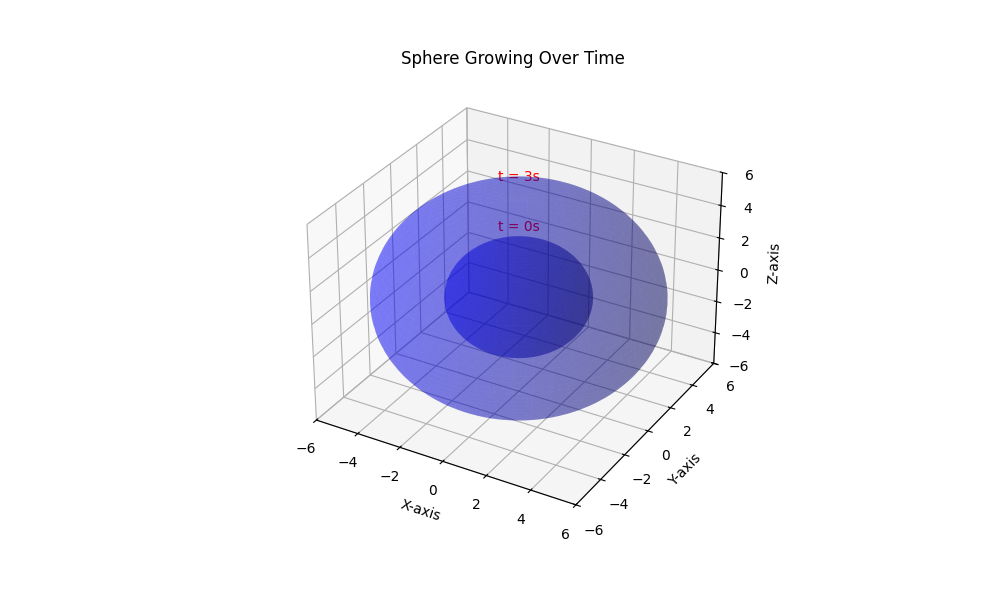
\includegraphics[width=0.7\textwidth]{figs/growing_sphere.png}
    \caption{Visualization of the sphere growing over time.}
\end{figure}

\textbf{Python Code To Calculate Radius:}
\begin{lstlisting}[language=Python]
import numpy as np
def calculate_radius(r_0, r_3, t):
    t_0 = 3.0  #Time at which r_3 is given (in seconds) 
    rate = 4*(np.pi)*(r_3**3 - r_0**3)/(3*t_0) #Calculate the rate of change of volume
    r_t = ((r_0**3) + (3*rate*t)/(4*np.pi))**(1/3) #Calculate the radius at time t
    return r_t
try:
    r_0 = float(input("Enter initial radius (r_0): "))
    r_3 = float(input("Enter radius at 3 seconds (r_3): "))
    t = float(input("Enter the time (t) after which the radius is to be found: "))
    if r_0 <= 0 or r_3 <= 0 or t < 0:
        print("All radii must be positive, and time must be non-negative.")
    else:
        r_t = calculate_radius(r_0, r_3, t)
        print(f"The radius of the sphere after {t} seconds is {r_t:.3f} units.")
except ValueError:
    print("Invalid input. Please enter numeric values.")
\end{lstlisting}

\end{document}
